Marcelo prepara brochetas como la siguiente con palitos y trozos de salchichas:

\begin{minipage}{0.4\linewidth}
    \begin{figure}[H]
        \centering
        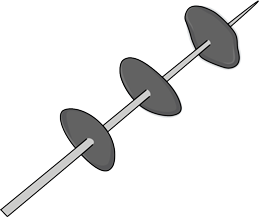
\includegraphics[width=0.9\linewidth]{../images/8cc56669378bdf27d863fffcaffb0080db06805e}
        \caption{Brocheta demostrativa}
        \label{fig:8cc56669378bdf27d863fffcaffb0080db06805e}
    \end{figure}
\end{minipage}\hfill
\begin{minipage}{0.6\linewidth}
    Para calcular cuántos palitos y cuántos trozos de salchicha necesitará, Marcelo elabora la siguiente tabla:

    \begin{table}[H]
        \centering
        \caption{}
        \label{tab:estampillas}
        \begin{tabular}{c|c|c|c|c|c|c}
            Cantidad de palitos             & 1 & 2 & 3 & 4  & \dots & 20 \\ \hline
            Cantidad de trozos de salchicha & 3 & 6 & 9 & 12 & \dots &    \\
        \end{tabular}
    \end{table}


    Si Marcelo cuenta la cantidad de trozos de salchicha que necesita para preparar
    20 palitos y luego suma todos los trozos que figuran en su tabla,
    \textbf{¿cuántos trozos obtendrá?}

    \begin{solutionbox}{1.2cm}
        630 trozos.
    \end{solutionbox}

\end{minipage}